% !TEX encoding = UTF-8
% !TEX TS-program = pdflatex
% !TEX root = ../tesi.tex

%**************************************************************
\chapter{Progettazione e sviluppo}
\label{cap:progettazione}
%**************************************************************

\section{Progettazione}
\subsection{Architettura}

Prima di descrivere la varie aggiunte che sono state apportate al software è necessario fornire un'idea dell'architettura sulla quale il progetto si basa.In questo modo si 
rendono più chiare molte delle scelte che sono state prese e il perchè altre sono state scartate. Di seguito è presentato uno schema ad alto livello di come sono strutturate le
varie componenti che formano l'intero sistema. Come possiamo notare dalla figura sottostante, il progetto segue un flusso pressochè "ciclico", partendo dal recupero dei dati dal
database e infine fornendo la soluzione. I dati estratti dal database vengono convertiti in file JSON il quale verrà letto dall'algoritmo che ha il compito di trovare la soluzione,
una volta fornita la soluzione essa viene ritradotta in un file JSON il quale viene letto e trasposto nell'interfaccia utente.

\begin{figure}[H]
	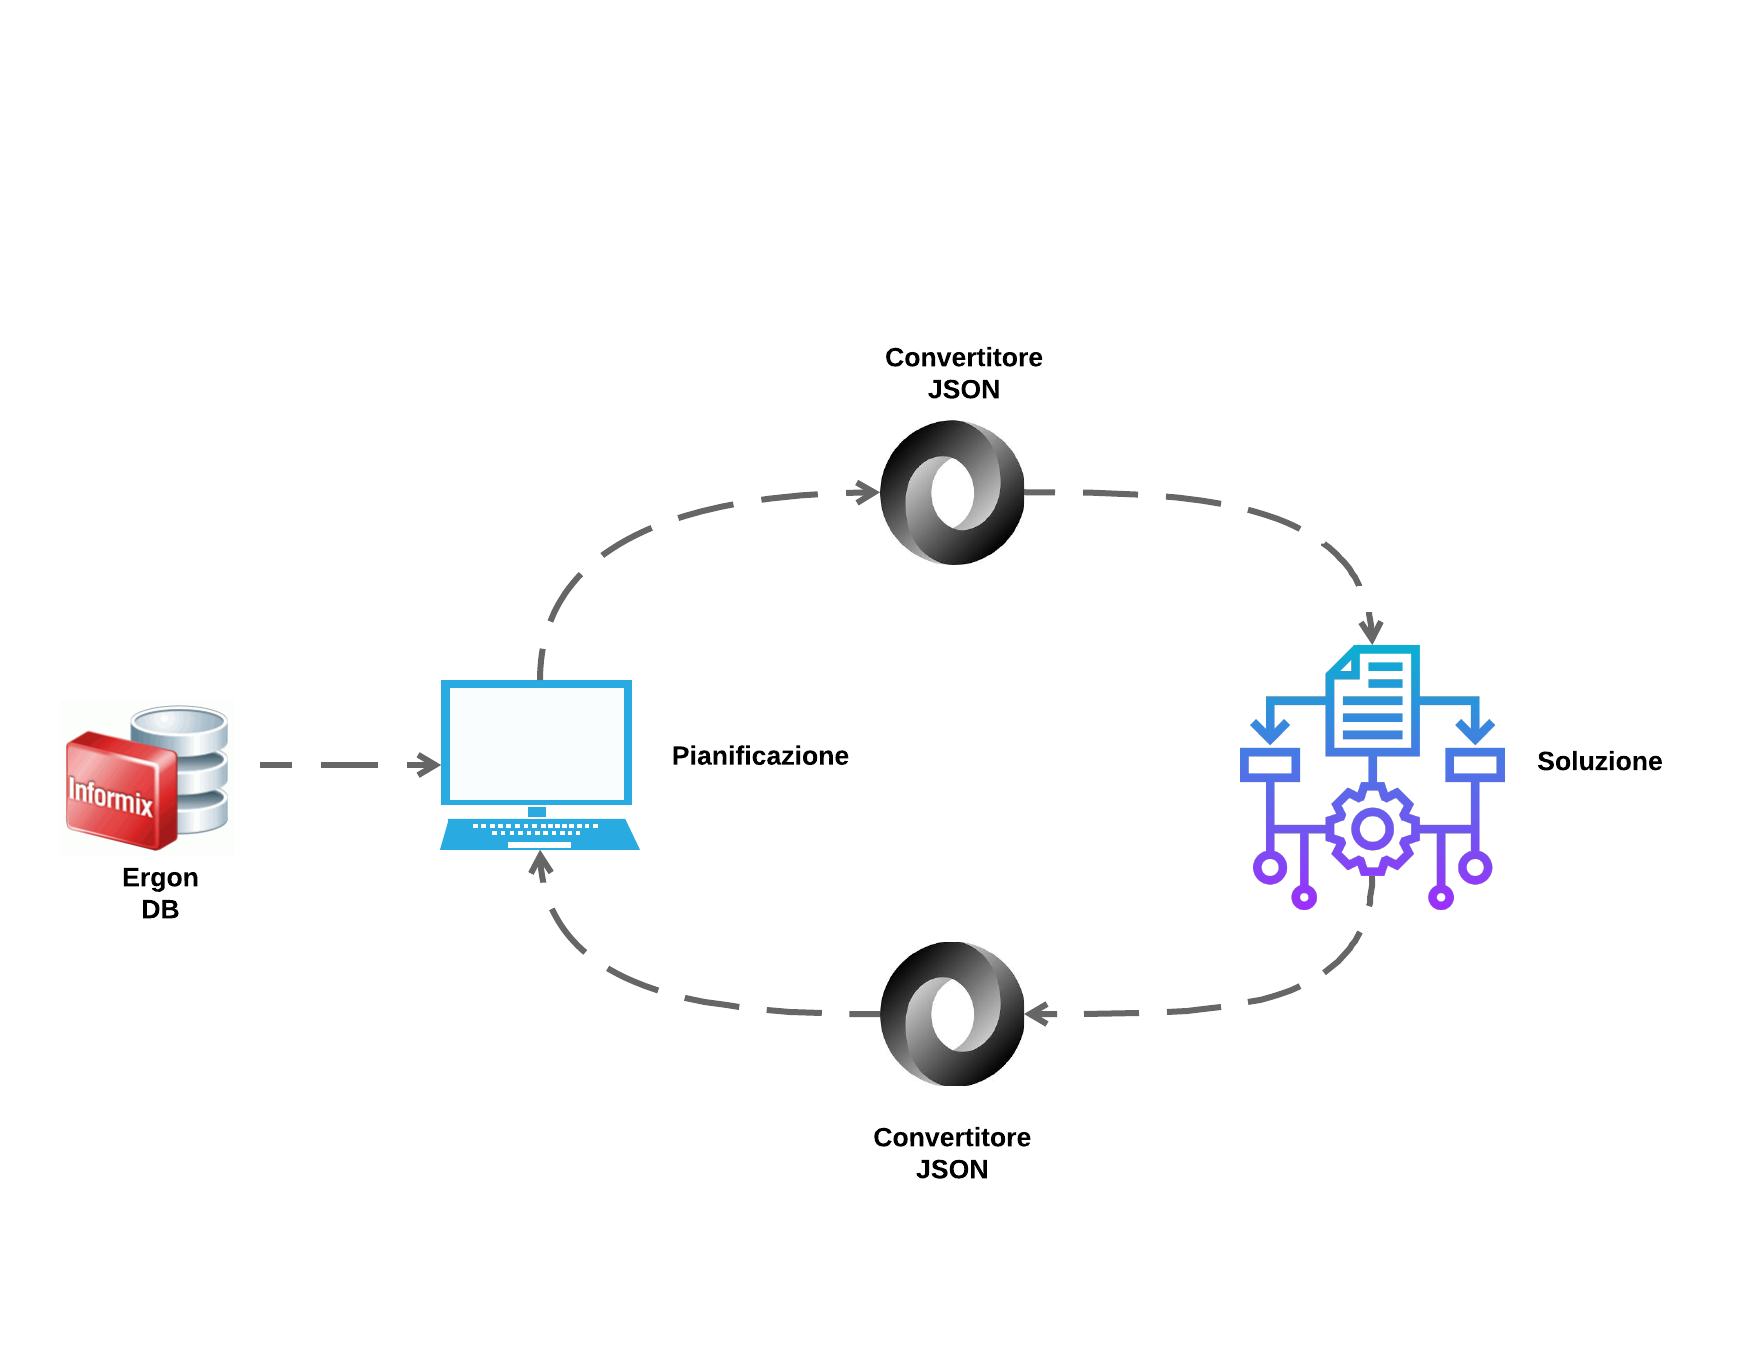
\includegraphics[width=10cm]{immagini/architettura.png}
	\centering
	\caption{Architettura generale}
\end{figure}

\subsection{Algoritmo}

\textbf{Il problema}

Dovendo integrare delle nuove funzionalità al programma esistente, si è prima effettuata un analisi del problema esistente per quanto riguarda la pianificazione della produzione,
in modo da poter comprendere alcune delle scelte euristiche\glosp che sono state effettuate in seguito.
Il suddetto problema rientra nella categoria NP-hard\glosp in quanto è riconducibile al problema del commesso viaggiatore\glo. A tali problemi non è possibile far corrispondere
una soluzione ottima ma, al massimo, la miglior approssimazione possibile di una soluzione ammissibile. In aggiunta al problema del commesso viaggiatore si devono considerare
altri vincoli come: 
\begin{itemize}
    \item tempo massimo sul quale si vogliono pianificare gli ordini;
    \item numero di linee sulle quali si possono produrre determinati ordini;
    \item vincoli generali di sequenza che andremo a definire in seguito.
\end{itemize}

Questo è l'insieme di problematiche riguardanti la precedente fase del progetto, dove rientrava solo la pianificazione dei prodotti finiti.
Con la richiesta di estendere tale progetto, il numero di vincoli da soddisfare cresce in proporzione al numero di ordini che si vogliono pianificare.
In particolare vanno tenuti in considerazione i vincoli precedenti più l'aggiunta dei seguenti:

\begin{itemize}
    \item pianificazione dei semilavorati antecedente ai prodotti finiti;
    \item materie prime e semilavorati presenti in quantità sufficienti per la produzione;
    \item verfica della disponibilità di materie prime e semilavorati in base agli ordini fornitori.
\end{itemize}

In conclusione, il problema che il progetto si pone di risolvere, consiste nel trovare una soluzione ammissibile, quanto più vicina all'ottimo,
della pianificazione
in base ai vincoli imposti.\newline

\textbf{La soluzione}

Dovendo appoggiarsi all'algoritmo esistente, non è stato possibile eseguire uno stravolgimento completo del suo funzionamento, anzi si è cercato di inserire le nuove funzionalità
in modo da integrarle il più possibile senza effettuare modifiche sostanziali alla struttura del codice esistente. Per fare ciò si è fatto ampio uso di nuove funzioni e classi, per poter
delegare, dalla base esistente, l'esecuzione di nuovi moduli di pianificazione. La struttura di partenza sulla quale vengono integrati i nuovi moduli è composta da un iniziale
fase di lettura dei dati dal database. Tali dati vengono convertiti in un file JSON che, per comodità di esecuzione, viene letto nuovamente dallo stesso programma, anche se
l'dea di base sarebbe quella di delegare la sua lettura e successiva elaborazione dei dati ad un sistema centralizzato esterno all'azienda che fornisce i dati stessi.
Una volta ottenuti i dati in formato JSON, vengono inseriti nell'algoritmo tramite l'impiego di classi e strutture predisposte. Tali classi vengono utilizzate come parametri
per la prima funzione che si pone come obiettivo quello di fornire una soluzione ammissibile nel minor tempo possibile ovvero l'Algoritmo Greedy\glo. Tale algoritmo ha il compito
di valutare, in modo sequenziale, i vari ordini che necessitano di essere pianificati, se un ordine soddisfa i vincoli imposti allora verrà inserito nella soluzione iniziale.
Una volta ottenuta la soluzione iniziale, questa viene fornita alla successiva funzione di ottimizzazione, composta da un algoritmo di Tabu Search\glo. Tale algoritmo ha il compito
di eseguire un insieme di mosse specifiche in modo casuale, valutando di volta in volta la bontà della soluzione ottenuta dopo la sua esecuzione. Al termine di un numero prefissato
di iterazioni, o dopo aver soddisfatto i criteri di aspirazione, verrà fornita la soluzione ottimizzata da visualizzare.
Visto che le scelte implementative non sempre possono essere chiare o si potrebbe pensare di utilizzare una metodologia diversa, viene illustrato di seguito il funzionamento
degli algoritmi su cui fa affidamento la pianificazione della produzione.\\

\textbf{Algoritmo Greedy}

È il primo passo per ottenere una soluzione ammissibile del problema in questione. Tale algoritmo si sviluppa tenendo conto che non è possibile effettuare dei "passi indietro",
ovvero, una volta inserito un ordine in pianificazione tale ordine rimane fino alla fine dell'esecuzione. I parametri in ingresso di tale algoritmo sono i seguenti:
\begin{itemize}
    \item ordini da pianificare;
    \item materie prime e semilavorati presenti in magazzino;
    \item materie prime e semilavorati presenti in ordini fornitori;
    \item linee di lavorazione con i rispettivi vincoli.
\end{itemize}

L'ordine di funzionamento è quindi il seguente:

\begin{itemize}
    \item prima scelta euristica, vengono ordinati i prodotti in base alla loro data di spedizione;
    \item il primo ordine in questione viene valutato;
    \item si verifica la presenza di materie prime, e qui abbiamo i seguenti casi:
            \begin{itemize}
                \item le materie prime sono disponibili per produrre l'ordine, inserisco in pianificazione;
                \item le materie prime non sono disponibili per produrre l'ordine, verifico l'arrivo di eventuali materie prime da parte dei fornitori,
                 se ciò avviene inserisco in pianificazione;
                \item non pianifico l'ordine.
            \end{itemize}
    \item si verifica la presenza di semilavorati, e qui abbiamo i seguenti casi:
            \begin{itemize}
                \item i semilavorati sono disponibili per produrre l'ordine, inserisco in pianificazione;
                \item i semilavorati non sono disponibili per produrre l'ordine, provo ad eseguire la pianificazione dei semilavorati mancanti, se ciò avviene
                inserisco in pianificazione;
                \item non pianifico l'ordine.
            \end{itemize}
    \item ogni valutazione effettua un controllo se è possibile inserire l'ordine in base al tempo lavorativo rimanente;
    \item si ripetono le azioni sopracitate fino al termine della valutazione di tutti gli ordini da pianificare.
\end{itemize}

Si ricorda che non è necessario che tutti gli ordini richiesti siano pianificati in quanto uno dei precedenti vincoli può non essere soddisfatto e, se tale ordine venisse
inserito nella soluzione, quest'ultima sarebbe non ammissibile perché viola appunto almeno uno dei vincoli imposti. Inoltre, se si esegue un accurato controllo, si può notare che 
il risultato fornito al termine della sua esecuzione, in alcuni casi, ha un ampio margine di miglioramento. L'algoritmo Greedy ha come obiettivo quello di creare una
soluzione iniziale nel modo più rapido possibile, in modo da avere una base di partenza per la successiva ottimizzazione eseguita dall'algoritmo Tabu Search.
